% Also note that the "draftcls" or "draftclsnofoot", not "draft", option
% should be used if it is desired that the figures are to be displayed in
% draft mode.
%
\documentclass[conference]{IEEEtran}
\makeatletter
\long\def\@makecaption#1#2{\ifx\@captype\@IEEEtablestring%
\footnotesize\begin{center}{\normalfont\footnotesize #1}\\
{\normalfont\footnotesize\scshape #2}\end{center}%
\@IEEEtablecaptionsepspace
\else
\@IEEEfigurecaptionsepspace
\setbox\@tempboxa\hbox{\normalfont\footnotesize {#1.}~~ #2}%
\ifdim \wd\@tempboxa >\hsize%
\setbox\@tempboxa\hbox{\normalfont\footnotesize {#1.}~~ }%
\parbox[t]{\hsize}{\normalfont\footnotesize \noindent\unhbox\@tempboxa#2}%
\else
\hbox to\hsize{\normalfont\footnotesize\hfil\box\@tempboxa\hfil}\fi\fi}
\makeatother
% Add the compsoc option for Computer Society conferences.
%
% If IEEEtran.cls has not been installed into the LaTeX system files,
% manually specify the path to it like:
% \documentclass[conference]{../sty/IEEEtran}

% Some very useful LaTeX packages include:
% (uncomment the ones you want to load)


% *** MISC UTILITY PACKAGES ***
%
%\usepackage{ifpdf}
% Heiko Oberdiek's ifpdf.sty is very useful if you need conditional
% compilation based on whether the output is pdf or dvi.
% usage:
% \ifpdf
%   % pdf code
% \else
%   % dvi code
% \fi
% The latest version of ifpdf.sty can be obtained from:
% http://www.ctan.org/tex-archive/macros/latex/contrib/oberdiek/
% Also, note that IEEEtran.cls V1.7 and later provides a builtin
% \ifCLASSINFOpdf conditional that works the same way.
% When switching from latex to pdflatex and vice-versa, the compiler may
% have to be run twice to clear warning/error messages.


% *** CITATION PACKAGES ***
%
\usepackage{cite}
% cite.sty was written by Donald Arseneau
% V1.6 and later of IEEEtran pre-defines the format of the cite.sty package
% \cite{} output to follow that of IEEE. Loading the cite package will
% result in citation numbers being automatically sorted and properly
% "compressed/ranged". e.g., [1], [9], [2], [7], [5], [6] without using
% cite.sty will become [1], [2], [5]--[7], [9] using cite.sty. cite.sty's
% \cite will automatically add leading space, if needed. Use cite.sty's
% noadjust option (cite.sty V3.8 and later) if you want to turn this off.
% cite.sty is already installed on most LaTeX systems. Be sure and use
% version 4.0 (2003-05-27) and later if using hyperref.sty. cite.sty does
% not currently provide for hyperlinked citations.
% The latest version can be obtained at:
% http://www.ctan.org/tex-archive/macros/latex/contrib/cite/
% The documentation is contained in the cite.sty file itself.


% *** GRAPHICS RELATED PACKAGES ***
%
\ifCLASSINFOpdf
   \usepackage[pdftex]{graphicx}
  % declare the path(s) where your graphic files are
  % \graphicspath{{../pdf/}{../jpeg/}}
  % and their extensions so you won't have to specify these with
  % every instance of \includegraphics
  % \DeclareGraphicsExtensions{.pdf,.jpeg,.png}
\else
  % or other class option (dvipsone, dvipdf, if not using dvips). graphicx
  % will default to the driver specified in the system graphics.cfg if no
  % driver is specified.
  % \usepackage[dvips]{graphicx}
  % declare the path(s) where your graphic files are
  % \graphicspath{{../eps/}}
  % and their extensions so you won't have to specify these with
  % every instance of \includegraphics
  % \DeclareGraphicsExtensions{.eps}
\fi
% graphicx was written by David Carlisle and Sebastian Rahtz. It is
% required if you want graphics, photos, etc. graphicx.sty is already
% installed on most LaTeX systems. The latest version and documentation can
% be obtained at: 
% http://www.ctan.org/tex-archive/macros/latex/required/graphics/
% Another good source of documentation is "Using Imported Graphics in
% LaTeX2e" by Keith Reckdahl which can be found as epslatex.ps or
% epslatex.pdf at: http://www.ctan.org/tex-archive/info/
%
% latex, and pdflatex in dvi mode, support graphics in encapsulated
% postscript (.eps) format. pdflatex in pdf mode supports graphics
% in .pdf, .jpeg, .png and .mps (metapost) formats. Users should ensure
% that all non-photo figures use a vector format (.eps, .pdf, .mps) and
% not a bitmapped formats (.jpeg, .png). IEEE frowns on bitmapped formats
% which can result in "jaggedy"/blurry rendering of lines and letters as
% well as large increases in file sizes.
%
% You can find documentation about the pdfTeX application at:
% http://www.tug.org/applications/pdftex


% *** MATH PACKAGES ***
%
%\usepackage[cmex10]{amsmath}
% A popular package from the American Mathematical Society that provides
% many useful and powerful commands for dealing with mathematics. If using
% it, be sure to load this package with the cmex10 option to ensure that
% only type 1 fonts will utilized at all point sizes. Without this option,
% it is possible that some math symbols, particularly those within
% footnotes, will be rendered in bitmap form which will result in a
% document that can not be IEEE Xplore compliant!
%
% Also, note that the amsmath package sets \interdisplaylinepenalty to 10000
% thus preventing page breaks from occurring within multiline equations. Use:
%\interdisplaylinepenalty=2500
% after loading amsmath to restore such page breaks as IEEEtran.cls normally
% does. amsmath.sty is already installed on most LaTeX systems. The latest
% version and documentation can be obtained at:
% http://www.ctan.org/tex-archive/macros/latex/required/amslatex/math/


% *** SPECIALIZED LIST PACKAGES ***
%
%\usepackage{algorithmic}
% algorithmic.sty was written by Peter Williams and Rogerio Brito.
% This package provides an algorithmic environment fo describing algorithms.
% You can use the algorithmic environment in-text or within a figure
% environment to provide for a floating algorithm. Do NOT use the algorithm
% floating environment provided by algorithm.sty (by the same authors) or
% algorithm2e.sty (by Christophe Fiorio) as IEEE does not use dedicated
% algorithm float types and packages that provide these will not provide
% correct IEEE style captions. The latest version and documentation of
% algorithmic.sty can be obtained at:
% http://www.ctan.org/tex-archive/macros/latex/contrib/algorithms/
% There is also a support site at:
% http://algorithms.berlios.de/index.html
% Also of interest may be the (relatively newer and more customizable)
% algorithmicx.sty package by Szasz Janos:
% http://www.ctan.org/tex-archive/macros/latex/contrib/algorithmicx/


% *** ALIGNMENT PACKAGES ***
%
%\usepackage{array}
% Frank Mittelbach's and David Carlisle's array.sty patches and improves
% the standard LaTeX2e array and tabular environments to provide better
% appearance and additional user controls. As the default LaTeX2e table
% generation code is lacking to the point of almost being broken with
% respect to the quality of the end results, all users are strongly
% advised to use an enhanced (at the very least that provided by array.sty)
% set of table tools. array.sty is already installed on most systems. The
% latest version and documentation can be obtained at:
% http://www.ctan.org/tex-archive/macros/latex/required/tools/


%\usepackage{mdwmath}
%\usepackage{mdwtab}
% Also highly recommended is Mark Wooding's extremely powerful MDW tools,
% especially mdwmath.sty and mdwtab.sty which are used to format equations
% and tables, respectively. The MDWtools set is already installed on most
% LaTeX systems. The lastest version and documentation is available at:
% http://www.ctan.org/tex-archive/macros/latex/contrib/mdwtools/


% IEEEtran contains the IEEEeqnarray family of commands that can be used to
% generate multiline equations as well as matrices, tables, etc., of high
% quality.


%\usepackage{eqparbox}
% Also of notable interest is Scott Pakin's eqparbox package for creating
% (automatically sized) equal width boxes - aka "natural width parboxes".
% Available at:
% http://www.ctan.org/tex-archive/macros/latex/contrib/eqparbox/


% *** SUBFIGURE PACKAGES ***
%\usepackage[tight,footnotesize,caption=false]{subfig}
\usepackage[caption=false]{subfig}
%\usepackage[center]{caption}
% subfigure.sty was written by Steven Douglas Cochran. This package makes it
% easy to put subfigures in your figures. e.g., "Figure 1a and 1b". For IEEE
% work, it is a good idea to load it with the tight package option to reduce
% the amount of white space around the subfigures. subfigure.sty is already
% installed on most LaTeX systems. The latest version and documentation can
% be obtained at:
% http://www.ctan.org/tex-archive/obsolete/macros/latex/contrib/subfigure/
% subfigure.sty has been superceeded by subfig.sty.
% subfig.sty, also written by Steven Douglas Cochran, is the modern
% replacement for subfigure.sty. However, subfig.sty requires and
% automatically loads Axel Sommerfeldt's caption.sty which will override
% IEEEtran.cls handling of captions and this will result in nonIEEE style
% figure/table captions. To prevent this problem, be sure and preload
% caption.sty with its "caption=false" package option. This is will preserve
% IEEEtran.cls handing of captions. Version 1.3 (2005/06/28) and later 
% (recommended due to many improvements over 1.2) of subfig.sty supports
% the caption=false option directly:
%\usepackage[caption=false,font=footnotesize]{subfig}
%
% The latest version and documentation can be obtained at:
% http://www.ctan.org/tex-archive/macros/latex/contrib/subfig/
% The latest version and documentation of caption.sty can be obtained at:
% http://www.ctan.org/tex-archive/macros/latex/contrib/caption/


% *** FLOAT PACKAGES ***
%
\usepackage{fixltx2e}
% fixltx2e, the successor to the earlier fix2col.sty, was written by
% Frank Mittelbach and David Carlisle. This package corrects a few problems
% in the LaTeX2e kernel, the most notable of which is that in current
% LaTeX2e releases, the ordering of single and double column floats is not
% guaranteed to be preserved. Thus, an unpatched LaTeX2e can allow a
% single column figure to be placed prior to an earlier double column
% figure. The latest version and documentation can be found at:
% http://www.ctan.org/tex-archive/macros/latex/base/


\usepackage{stfloats}
% stfloats.sty was written by Sigitas Tolusis. This package gives LaTeX2e
% the ability to do double column floats at the bottom of the page as well
% as the top. (e.g., "\begin{figure*}[!b]" is not normally possible in
% LaTeX2e). It also provides a command:
%\fnbelowfloat
% to enable the placement of footnotes below bottom floats (the standard
% LaTeX2e kernel puts them above bottom floats). This is an invasive package
% which rewrites many portions of the LaTeX2e float routines. It may not work
% with other packages that modify the LaTeX2e float routines. The latest
% version and documentation can be obtained at:
% http://www.ctan.org/tex-archive/macros/latex/contrib/sttools/
% Documentation is contained in the stfloats.sty comments as well as in the
% presfull.pdf file. Do not use the stfloats baselinefloat ability as IEEE
% does not allow \baselineskip to stretch. Authors submitting work to the
% IEEE should note that IEEE rarely uses double column equations and
% that authors should try to avoid such use. Do not be tempted to use the
% cuted.sty or midfloat.sty packages (also by Sigitas Tolusis) as IEEE does
% not format its papers in such ways.



% *** PDF, URL AND HYPERLINK PACKAGES ***
%
\usepackage{url}
% url.sty was written by Donald Arseneau. It provides better support for
% handling and breaking URLs. url.sty is already installed on most LaTeX
% systems. The latest version can be obtained at:
% http://www.ctan.org/tex-archive/macros/latex/contrib/misc/
% Read the url.sty source comments for usage information. Basically,
% \url{my_url_here}.


\usepackage{listings}

% correct bad hyphenation here
\hyphenation{op-tical net-works semi-conduc-tor}

\pagestyle{plain}

\begin{document}

\lstset{basicstyle=\footnotesize}

%
% paper title
% can use linebreaks \\ within to get better formatting as desired
\title{Security Audit of Safeplug ``Tor in a Box''}


% author names and affiliations
% use a multiple column layout for up to three different
% affiliations
%\author{\IEEEauthorblockN{Anne Edmundson}
%\IEEEauthorblockA{Department of Computer Science\\
%Princeton University\\
%Princeton, New Jersey 08540-5233\\
%Email: annee@cs.princeton.edu}
%\and
%\IEEEauthorblockN{Anna Kornfeld Simpson}
%\IEEEauthorblockA{Department of Computer Science\\
%Princeton University\\
%Princeton, New Jersey 08540-5233\\
%Email: aksimpso@cs.princeton.edu}
%\and
%\IEEEauthorblockN{Josh Kroll}
%\IEEEauthorblockA{Department of Computer Science\\
%Princeton University\\
%Princeton, New Jersey 08540-5233\\
%Email: kroll@cs.princeton.edu}
%\and
%\IEEEauthorblockN{Ed Felten}
%\IEEEauthorblockA{Department of Computer Science\\
%Princeton University\\
%Princeton, New Jersey 08540-5233\\
%Email: felten@cs.princeton.edu}}

% conference papers do not typically use \thanks and this command
% is locked out in conference mode. If really needed, such as for
% the acknowledgment of grants, issue a \IEEEoverridecommandlockouts
% after \documentclass

% for over three affiliations, or if they all won't fit within the width
% of the page, use this alternative format:
% 
\author{\IEEEauthorblockN{Anna Kornfeld Simpson,
Anne Edmundson,
Josh Kroll, and
Ed Felten}
\IEEEauthorblockA{Department of Computer Science\\
Princeton University,
Princeton, NJ 08540-5233}}


% use for special paper notices
%\IEEEspecialpapernotice{(Invited Paper)}


% make the title area
\maketitle


\begin{abstract}
%\boldmath
We present the first public third-party security audit of Pogoplug's Safeplug device, which marketed ``complete security and anonymity online'' by using Tor technology to protect users' IP addresses.  We examine the hardware, software, and network behavior of the Safeplug device, as well as the user experience in comparison to other forms of web browsing.  Although the Safeplug appears to use Tor as advertised, users may still be identified in ways they may not expect.  Furthermore, an engineering vulnerability in the Safeplug's settings commands would allow an adversary internal or external to a user's home network to silently disable Tor or modify other Safeplug settings, which completely overrules the security claims of the device.  Even if the engineering problem is fixed, the user experience challenges of this type of device make it inferior to the existing standard in anonymity methods: the Tor Browser Bundle.
\end{abstract}
% IEEEtran.cls defaults to using nonbold math in the Abstract.
% This preserves the distinction between vectors and scalars. However,
% if the conference you are submitting to favors bold math in the abstract,
% then you can use LaTeX's standard command \boldmath at the very start
% of the abstract to achieve this. Many IEEE journals/conferences frown on
% math in the abstract anyway.

% no keywords

% For peer review papers, you can put extra information on the cover
% page as needed:
% \ifCLASSOPTIONpeerreview
% \begin{center} \bfseries EDICS Category: 3-BBND \end{center}
% \fi
%
% For peerreview papers, this IEEEtran command inserts a page break and
% creates the second title. It will be ignored for other modes.
\IEEEpeerreviewmaketitle


% An example of a floating figure using the graphicx package.
% Note that \label must occur AFTER (or within) \caption.
% For figures, \caption should occur after the \includegraphics.
% Note that IEEEtran v1.7 and later has special internal code that
% is designed to preserve the operation of \label within \caption
% even when the captionsoff option is in effect. However, because
% of issues like this, it may be the safest practice to put all your
% \label just after \caption rather than within \caption{}.
%
% Reminder: the "draftcls" or "draftclsnofoot", not "draft", class
% option should be used if it is desired that the figures are to be
% displayed while in draft mode.
%
%\begin{figure}[!t]
%\centering
%\includegraphics[width=2.5in]{myfigure}
% where an .eps filename suffix will be assumed under latex, 
% and a .pdf suffix will be assumed for pdflatex; or what has been declared
% via \DeclareGraphicsExtensions.
%\caption{Simulation Results}
%\label{fig_sim}
%\end{figure}

% Note that IEEE typically puts floats only at the top, even when this
% results in a large percentage of a column being occupied by floats.


% An example of a double column floating figure using two subfigures.
% (The subfig.sty package must be loaded for this to work.)
% The subfigure \label commands are set within each subfloat command, the
% \label for the overall figure must come after \caption.
% \hfil must be used as a separator to get equal spacing.
%
%\begin{figure*}[!t]
%\centerline{\subfloat[Case I]\includegraphics[width=2.5in]{subfigcase1}%
%\label{fig_first_case}}
%\hfil
%\subfloat[Case II]{\includegraphics[width=2.5in]{subfigcase2}%
%\label{fig_second_case}}}
%\caption{Simulation results}
%\label{fig_sim}
%\end{figure*}
%
% Note that often IEEE papers with subfigures do not employ subfigure
% captions (using the optional argument to \subfloat), but instead will
% reference/describe all of them (a), (b), etc., within the main caption.


% An example of a floating table. Note that, for IEEE style tables, the 
% \caption command should come BEFORE the table. Table text will default to
% \footnotesize as IEEE normally uses this smaller font for tables.
% The \label must come after \caption as always.
%
%\begin{table}[!t]
%% increase table row spacing, adjust to taste
%\renewcommand{\arraystretch}{1.3}
% if using array.sty, it might be a good idea to tweak the value of
% \extrarowheight as needed to properly center the text within the cells
%\caption{An Example of a Table}
%\label{table_example}
%\centering
%% Some packages, such as MDW tools, offer better commands for making tables
%% than the plain LaTeX2e tabular which is used here.
%\begin{tabular}{|c||c|}
%\hline
%One & Two\\
%\hline
%Three & Four\\
%\hline
%\end{tabular}
%\end{table}


\section{Introduction}
% no \IEEEPARstart

Privacy on the Internet is becoming increasingly important as more users realize how vulnerable they are to surveillance and attacks; anonymity has become the goal for many Internet users in order to protect themselves.  A recent study has shown that people have been the victim of many security-related issues, such as compromised emails/accounts, harrassment, stolen Social Security Numbers, bank information, and credit card numbers, due to their online visibility~\cite{pew}.  As the Internet grows and the amount of user information that is collected and/or provided online increases, users will continue to be more vulnerable.  According to one study, 86\% of internet users have tried to become more anonymous online by either clearing cookies, encrypting their email, or using virtual networks that mask their IP address~\cite{pew}.  While this study shows that a large percentage of users are taking measures to reduce their visibility online, 59\% reported that they don't believe it is possible to become completely anonymous online~\cite{pew}.  

The cloud storage company Pogoplug noticed the demand for online anonymity and in December of 2013 they released the Safeplug.  This device is a small box that plugs into a user's home router and by routing all traffic through Tor, it claims to: conceal your identity, hide where you live, shield your surfing habits, and make you anonymous online~\cite{pogo}.  The Safeplug also claimed simple setup and an abstraction of any technical detail, as shown by the setup instructions that came with the device shown in Figure~\ref{fig:instructions}.  A device such as this should be audited to confirm or deny the validity of the bold security claims.  We conducted the first public third-party security audit of the Safeplug by analyzing the hardware, software, and network behavior.  The following are some of our findings:

\begin{itemize}
\item The Safeplug functions as a HTTP proxy for the browser, which then uses Tor on outgoing traffic (see Figure \ref{fig:flow}).
\item The browser collects both first- and third-party tracking cookies, de-anonymizing users across websites despite the presence of Tor.
\item A Safeplug user is vulnerable to a Cross-Site Request Forgery (CSRF) attack that allows an outside attacker to modify the Safeplug settings (i.e., turning Tor on/off, turning ad-blocking on/off, turning the Tor relay setting on/off, adding/removing whitelisted sites from Tor).
\item A malicious user within the network can modify the Safeplug settings without notifying any other devices on the network.
\item The Safeplug has a higher web request latency than that of the Tor Browser Bundle.
\end{itemize} 

Pogoplug made use of good security principles by using auditable open source software on their device, and has a laudable goal of making online security the standard for more users.  However, even if the engineering vulnerabilities are fixed with proper authentication for modifying Safeplug settings, the incompleteness of the provided anonymity and risks of adding an additional box to the trusted inside of the home network mean that there is little reason to use the Safeplug over the Tor Browser Bundle.

\begin{figure*}
\centering
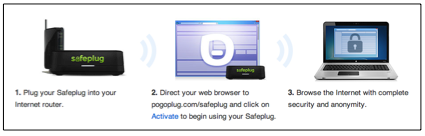
\includegraphics[width=.75\textwidth]{instructions2}
\caption{Setup instructions (and the only documentation) that came in the box with the Safeplug. Pogoplug highlights the ease of installing the device but does not give a clear indication of how the Safeplug functions.}
\label{fig:instructions}
\end{figure*}  

\begin{figure*}
\centering
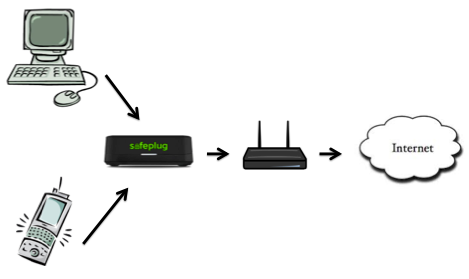
\includegraphics[width=.4\textwidth]{safeplug_flowchart}
\caption{Flowchart demonstrating the actual functionality of the Safeplug as an HTTP proxy between a device's browser and the home network's router.}
\label{fig:flow}
\end{figure*}  

\section{Background}
{\bf Tor.} The state-of-the-art in online anonymity technology is the open-source project Tor.  Tor is a service that provides anonymous communication as an onion router; by encrypting internet traffic and sending it through layers of relays, a user can make it much more difficult to trace their internet use~\cite{tor}.  Instead of appearing to come from a user's IP address, the traffic will reach the destination from one of the relays, that will have received the traffic from another relay, creating a chain back from when the user first sent their traffic to a relay.  Tor is known as an onion router because each relay peels back one layer of encryption and no more, allowing it to send the traffic to the next destination but not allowing it to discover the origin or final recipient of the traffic.  Tor is open-source software developed by the Tor Project~\cite{torproject}.  Users of Tor are highly recommended to use it as part of the Tor Browser Bundle, which provides a single installation of a browser and the Tor software package.  This browser has special settings to prevent deanonymization of the traffic by other means, such as cookies, supercookies, or scripts~\cite{torproject}.

Using Tor or the Tor Browser Bundle provides a tradeoff between anonymity, usability, and efficiency.  Sending traffic to these relays around the world slows down the traffic significantly, possibly degrading user experience for websites that load a lot of data in real-time.  In addition, because the destination website will see the user's request as coming from a new, likely international IP address, websites such as banks that have location-based safeguards may deny users access to their sites.  For many users around the world, these troubles are a worthwhile price for access to free and open internet, anonymous communications, and resisting censorship.  However, one of the biggest reasons that Tor is not more widespread is that many Internet users do not know about Tor, how it works, or how they would be able to use it to become more anonymous online.

{\bf Safeplug.} Safeplug is a product that launched in December of 2013 from the cloud storage company Pogoplug, that offers any user the option of using Tor without having to know about it or how it works.  It allows users to browse the web from their own standard web browser with “complete security and anonymity” for the cheap price of \$49 \cite{safeplug}.  Safeplug offers Tor out of the box, with no additional software installation, by sitting between a user's router and the Internet \cite{wired}.  Pogoplug's marketing pitch centers around the protection of users' IP addresses by using Tor \cite{safeplug,bittech}.

{\bf Pogoplug.} Pogoplug, a subsidary of Cloud Engines, also offers a box for home network file sharing without needing to use a third-party storage provider.  Based on our examination of the box discussed below, we suspect that the Pogoplug hardware was relabelled as Safeplug and simply uses different software to achieve its newly branded purpose.

\section{Design and Operation of Safeplug}

\subsection{Information Prior to Using the Device: Terms of Service}
\label{tos}
The Terms of Service (TOS) contains three main points of interest: TOS updates, open source licensing information, and software updates.  First, the TOS are not presented to the user in the Safeplug package (the only information in the packaging were the instructions shown in Figure~\ref{fig:instructions}) or during the activation process, and are only available through a small link at the bottom of the Safeplug website\cite{safeplug}.  Although use of the Safeplug device purportedly constitutes acceptance of the TOS, most users are not likely to read the TOS even once.  However, Pogoplug suggests that users regularly review the TOS because they can update or change them at any time; this is standard language in TOS but not a good combination with them not being presented to the user.

Following good security and development practices, the Safeplug makes use of several pieces of Open Source software.  A standard term of many open source licenses states that a company that uses the open source software must list the software used and its license, as well as the open source code of their own software that uses the license.  The TOS contains a link to a page that would supposedly comply with this requirement: \url{http://pogoplug.com/home-en-developers-open-source.html} but the link is dead and instead the reader sees a 404 error \cite{safeplug}.  This dead link was noted by some members of the Tor-talk mailing list in November 2013 and has not been fixed as of Feburary 2014 \cite{tormailinglist}.  Pogoplug's open source page does exist at \url{https://pogoplug.com/opensource} and includes several pieces of software for the Safeplug: bootloader, Linux kernel, XCE kernel support driver, glibc, BusyBox, and a Safeplug source bundle.  However, there is no way to find this page from the Terms of Service.

The final area of interest was software updates on the device which will be ``automatically delivered'' to the user, but it is unclear whether there will be any notification~\cite{safeplug}.  Although a prompt updating mechanism is an important security feature for users who trust Pogoplug and their update servers (in fact the activation process seems designed for keeping the software up to date and it is concerning that this does not seem to uniformly occur as discussed in Section~\ref{versions}), other users might want to disable this functionality for fear of a malicious use of Pogoplug's servers or a spoofing attack (see Section \ref{dnsspoof}).  This is one of the many reasons why users who truly need security and anonymity should opt for the Tor Browser Bundle rather than adding the Safeplug to their network.

\subsection{Explanation of Tor Configuration Options}
\label{port9001}
One of Safeplug's configurations is the use of the device as a Tor relay node in the Tor network.  When the device is initially set up, the default setting is to not use it as a relay node.  

The settings page describes Tor in an extremely basic way:

\begin{quotation}
``Safeplug uses the Tor network to secure your Internet connection.  Tor works by routing your Internet through a series of random destinations, much like driving a twisty, complicated route to throw off someone who is following you, making it impossible for websites and organizations to identify the source or destination of Internet traffic.'' \cite{safeplug}
\end{quotation}

On the other hand, it describes the functionality of a Tor relay node in a much more technical manner:
\begin{quotation}
``Make the Tor network strong for everybody! Enabling Tor Relay allows your Safeplug to act as a relay point on the Tor network. The more Tor relays that join the Tor network, the faster and more robust Tor becomes, helping everybody be more secure online. \\ \\ NOTE: You must forward inbound traffic on port 9001 to [IP-of-Safeplug]. \\ For help configuring your router, click here.''
\cite{safeplug}
\end{quotation}

The link provided is to an advertisement-filled and not particularly reputable-looking website with no clear navigation to get to the necessary instructions.  

If the majority of users can only understand the simpler description, then they likely won't understand the description of a Tor relay node.  This could be a problem if users simply decide not to do anything with that setting (i.e. don't change the setting to use the Safeplug as a relay node).  In this case, there would be a large increase in use of the Tor network, yet most of the users are not giving back to it.

This could easily be remedied; Safeplug should choose a target audience and have consistent descriptions.  The best option is to explain the Tor network and the functionality of a Tor relay node at the same level, preferably a level that normal Internet users can understand.  This increases the chances that users will run their Safeplug as a relay node.

Another consequence of misunderstanding the use of the Safeplug as a relay node, or more specifically, as an exit node is the possible legal repercussions.  As an exit relay, all traffic that exits the node can be traced back to the Safeplug's IP address; it is likely that some of this traffic contains illegal information or is part of illegal activities.  The Tor Project recommends not running an exit relay from a user's home: ``If law enforcement becomes interested in traffic from your exit relay, it's possible that officers will seize your computer. For that reason, it's best not to run your exit relay in your home or using your home Internet connection~\cite{law}.''  Considering that the Safeplug is intended for home use, it is a poor design choice to allow the user to use it as an exit relay, especially without providing the user with any information.

\subsection{Hardware}
Before investigating the software, we took apart one of the two Safeplug devices we purchased in order to see the physical components.  Figure~\ref{fig:top} shows the top of the board and Figure~\ref{fig:bottom} shows the bottom.  The board incorporates: (A) an SD card slot, (B) a power connector, (C) a USB slot, (D) an ethernet connector, (E) ethernet transceiver, (F) lan transformer, (G) the Marvell 88F6192 integrated controller, and (H), (I) flash memory.  The Marvell controller is from 2008 and runs ARM~\cite{marvellhw}. This is the same controller as version 4 of Pogoplug's cloud storage device; takedowns of that device that are available online show an identical-looking circuit-board to the one in Figure~\ref{fig:circuit}\cite{pogo4}.  It is also interesting to note that the Safeplug branding is a sticker on the front of the device, whereas the Pogoplug branding is etched into the plastic on top of the device, which indicates that the Safeplug uses the same hardware as Pogoplug's existing devices, and derives its differing functionality from different software.

\begin{figure*}[tb]
\centering
\subfloat[][Top of the board inside the Safeplug device.]{
  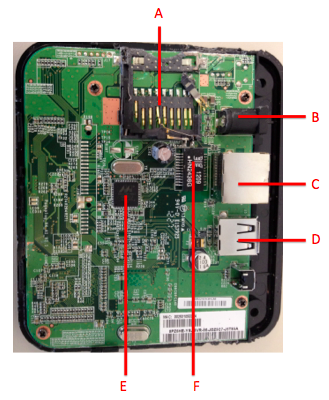
\includegraphics[width=.3\textwidth]{safeplug_listed_top}
  \label{fig:top}
}
\qquad
\subfloat[][Bottom of the Board inside the Safeplug device.]{
  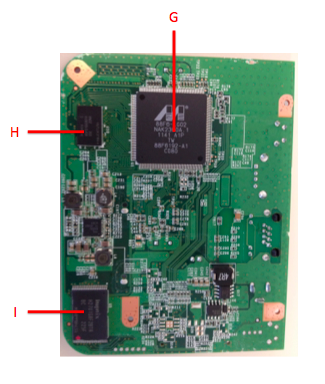
\includegraphics[width=.3\textwidth]{safeplug_hardware_new}
  \label{fig:bottom}
}
\caption{Safeplug circuit board after the teardown.}
\label{fig:circuit}
\end{figure*}

\subsection{Software on the Safeplug}
\label{versions}
\begin{center}
  \begin{tabular}{|l|c|c|}
    \hline
    Safeplug Software & Version & Date \\ \hline
    Linux Kernel & 2.6.31.8 & 2009 \\ \hline
    Lighttpd Web Server & 1.4.33 & 2013 \\ \hline
    Privoxy Proxy & 3.0.21 & 2013 \\ \hline
    Tor & 0.2.3.25 & 2012 \\ \hline
    Dropbear sshd & v0.52 & 2008 \\ \hline
  \end{tabular}
\end{center}

The Safeplug runs version 2.6.31.8 of Arch Linux on an ARM architecture, which was produced at the end of 2009 and installed on 23 August 2011.  Unsurprising for its age, there are a number of network vulnerabilities for this version of the kernel - most of which produce denial of service attacks if an adversary sends a particularly formed packet \cite{kernelcve}.  This is the same version of Linux that runs on Version 4 of Pogoplug's Mobile platform \cite{archforum}.

The software installed by the activation process on the Safeplug is in \verb!/opt/xce! and includes Lighttpd, Privoxy, and Tor.  Lighttpd is an open-source webserver, which is serving the settings page on the device - the project's description mentions ``security, speed, compliance, and flexibility [... while being] designed and optimized for high perfomance environments'' \cite{lighttpd}.  The version of Lighttpd on the box is only one version away from being up to date, 1.4.33 which was released on 27 September 2013.  The current version of Lighttpd, which has a number of security fixes, was released on 20 January 2014, after the Safeplug was purchased.  However, checking for an update from the Safeplug does not lead to any updated software installation.

Privoxy is a ``non-caching web proxy with advanced filtering capabilities for enhancing privacy, modifying webpage data and HTTP headers, controlling access, and removing ads and other obnoxious Internet junk'' and it specifically advertises its ``flexible configuration'' \cite{privoxy}.  Privoxy is also open source.  The version on the device is 3.0.21, which is the most recent release.

The version of Tor is v0.2.3.25 which is from November 2012.  The current stable version of Tor is v0.2.4.20 from December 2013.  Unlike Lighttpd and Privoxy, the Safeplug does not contain the most up-to-date version of Tor from when it was released.

The fourth piece of software discovered on the device, which is not installed during the activation process and is in \verb!/usr/sbin! is the Dropbear SSH server and client, used to support SSH access to the device \cite{dropbear}.  The Safeplug uses its own configuration files to determine how these pieces of software are set up and used.  The version of Dropbear on the Safeplug is v0.52 from 2008, which is extremely out of date.  Given the different location and installation methods, it seems likely that this was from the older Pogoplug device and is not designed to be updated in the same manner as the rest of the Safeplug software.  However, the SSH server is active and listening on port 22.

Figure \ref{fig:callgraph} shows the call graph for the modifying the settings page.  When a user modifies the settings page, Javascript on the settings page generates a POST request to xspctrl, which is running via CGI in Lighttpd. The CGI handler copies a number of environment variables and then forks and runs the xspctrl as execve (in the constructed environment). Xspctrl is a shell script which uses the end of the path to discover the correct method to run and executes any of the necessary binary files with specified arguments (go\_update, go\_upgrade, go\_sshd, or go\_updateexceptions) to complete its request before returning a response.

\begin{figure*}
\centering
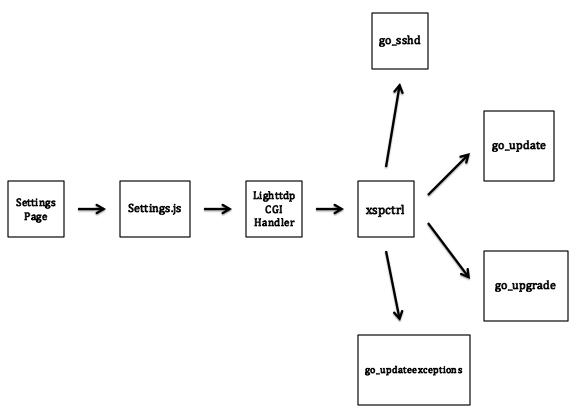
\includegraphics[width=.55\textwidth]{callgraph}
\caption{The call graph for modifying the Safeplug settings page.}
\label{fig:callgraph}
\end{figure*} 

\subsection{Networking}
The Lighttpd, Privoxy, and Dropbear software give some indication of the networking services on the device.  We used \texttt{nmap} to scan the ports.  Before the activation of the Safeplug, only ports 80 and 3333 are open.  After the activation, without the use of Tor turned on, port 22 for SSH, port 80 for settings access and port 8080 for http-proxy are open.  When Tor is turned on as a relay, port 9001 tor-orport is opened as well.  This corresponds with the note on the settings page about Tor relays discussed in Section \ref{port9001} above.
    
\subsection{Configuration on the Safeplug}
\label{spconfig}
The Safeplug configuration files can be found in \verb!/opt/xce/etc! and include \verb!sp.conf! and \verb!sp_version! and \verb!sp_torexceptions!.  The first contains all of the configuration details: whether to use Tor, whether to ad-block, and whether to be a relay or an exit relay. The version file is used during the check for updates, and the exceptions file is used by the Privoxy configuation to control the whitelist of sites not to connect to via Tor.

These configuration files are read by the scripts in \verb!/opt/xce/etc/init.d! which enable Lighttpd, Privoxy, and Tor.  As expected, Privoxy looks at the Tor, ad-block and exceptions configurations, and Tor reads the \verb!sp.conf! file to set which Tor configuration file (regular, relay, or exit relay) to use.

\section{Usability}
Several aspects of the user experience of the Safeplug affect the usability and security of the device.  The Safeplug advertisements highlighted the ease of setup and activation of the device.

\subsection{Activation and Setup}
The first step was to plug Safeplug into our router and activate our device.  Our instructions are shown in Figure~\ref{fig:instructions}.  We followed them, activated our device, and then ended on the configurations page.  The configurations page has a combination of platforms and browsers, with a different set of proxy configuration instructions for each one.  The platforms presented include popular desktop and mobile platforms.  The Tor Project has an Android application, as well as the Tor Browser Bundle for Windows and OSX (and Linux, which is not supported explicitly by Pogoplug's page but is likely to have a browser with similar configuration processes to Firefox).  However, there is no existing Tor Project application for iOS.

\begin{center}
	\begin{tabular}{|c|c|}
	\hline
		Platform & Browsers \\ \hline
		Windows	& Internet Explorer, Chrome, Firefox \\ \hline
		OSX & Safari, Chrome, Firefox \\ \hline
		iOS	& Safari \\ \hline
		Android	& Chrome \\ \hline
	\end{tabular}
\end{center}

After we finished our configuration, we were taken to the Safeplug settings page.  This page is shown in Figure~\ref{fig:settings}.  This allowed us to turn Tor on/off, add white-listed websites, turn ad-blocking on/off, and turn the ability of our device to be a relay node on/off (and if on, an additional option appeared to allow the device to be an exit node).  

\begin{figure}[htb]
  \centering
  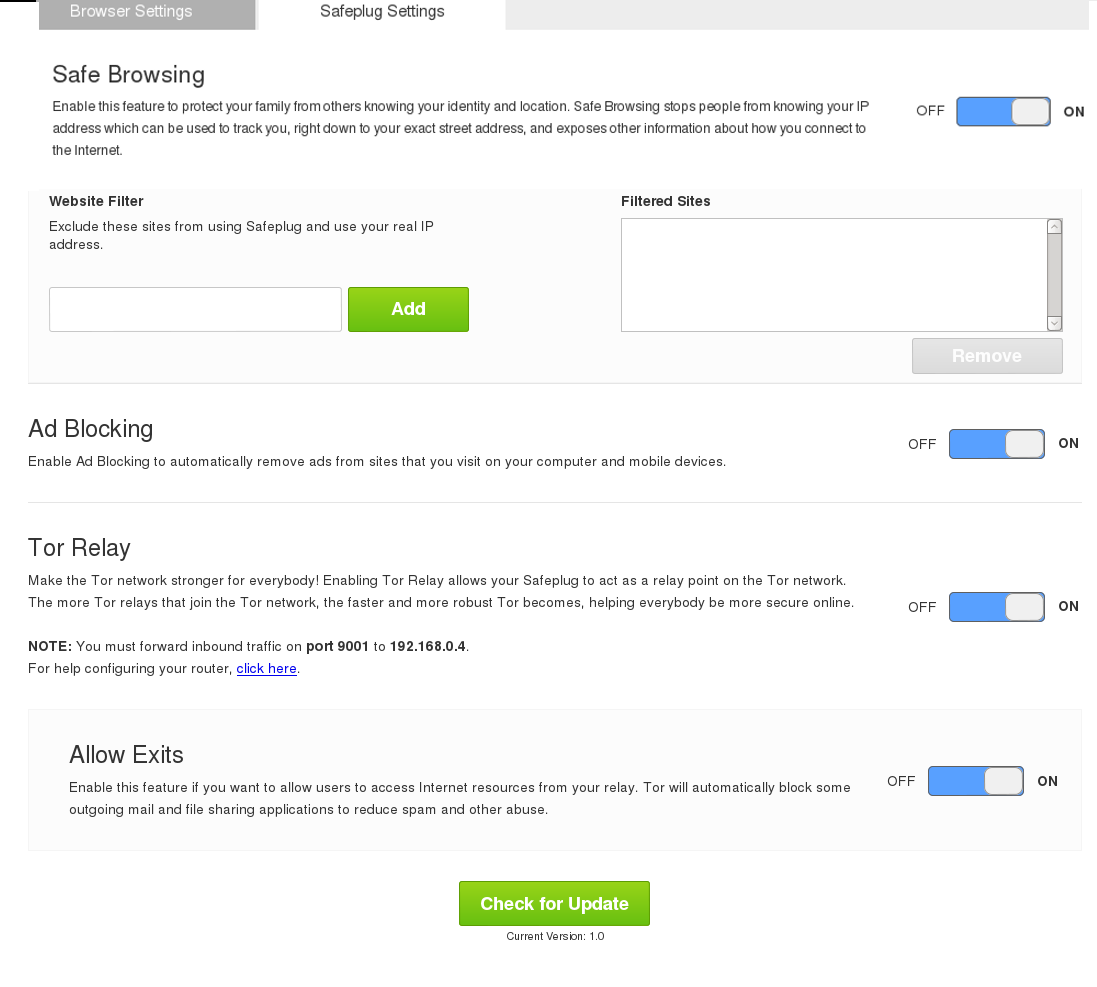
\includegraphics[width=.4\textwidth]{settings_with_exit}
  \caption{Safeplug settings page.  The last button ``Allow Exit'' only appears if the relay option above has been turned on.}
  \label{fig:settings}
\end{figure}

\subsection{Internet Use}
\label{inetuse}

\begin{figure*}[tb]
\centering
\subfloat[][Web page before using Tor and ad-blocking.]{
  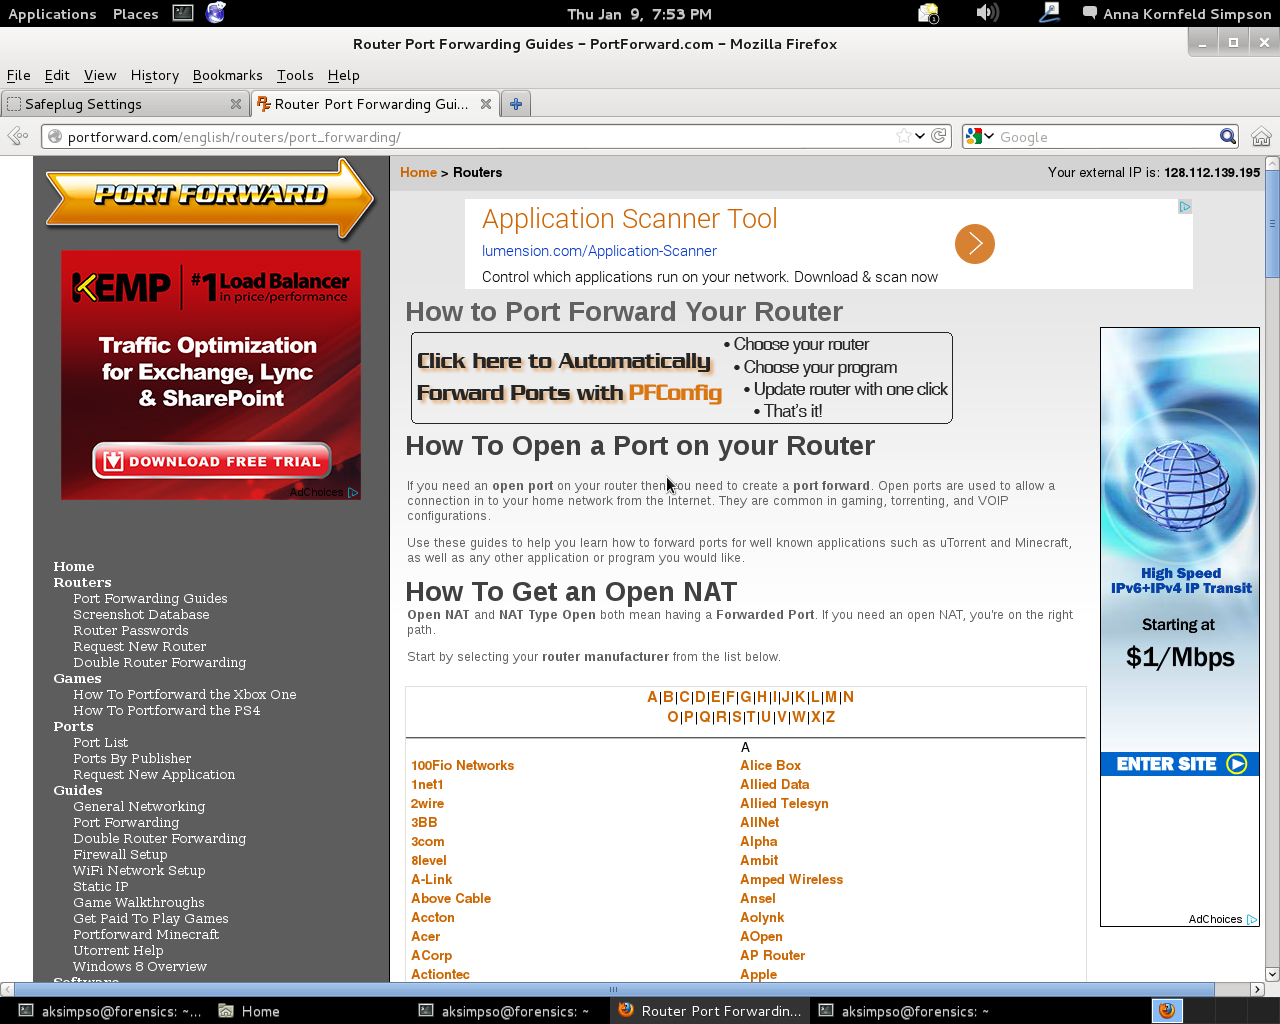
\includegraphics[width=.3\textwidth]{before}
  \label{fig:before}
}
\quad
\subfloat[][Web page after using Tor and ad-blocking.]{
  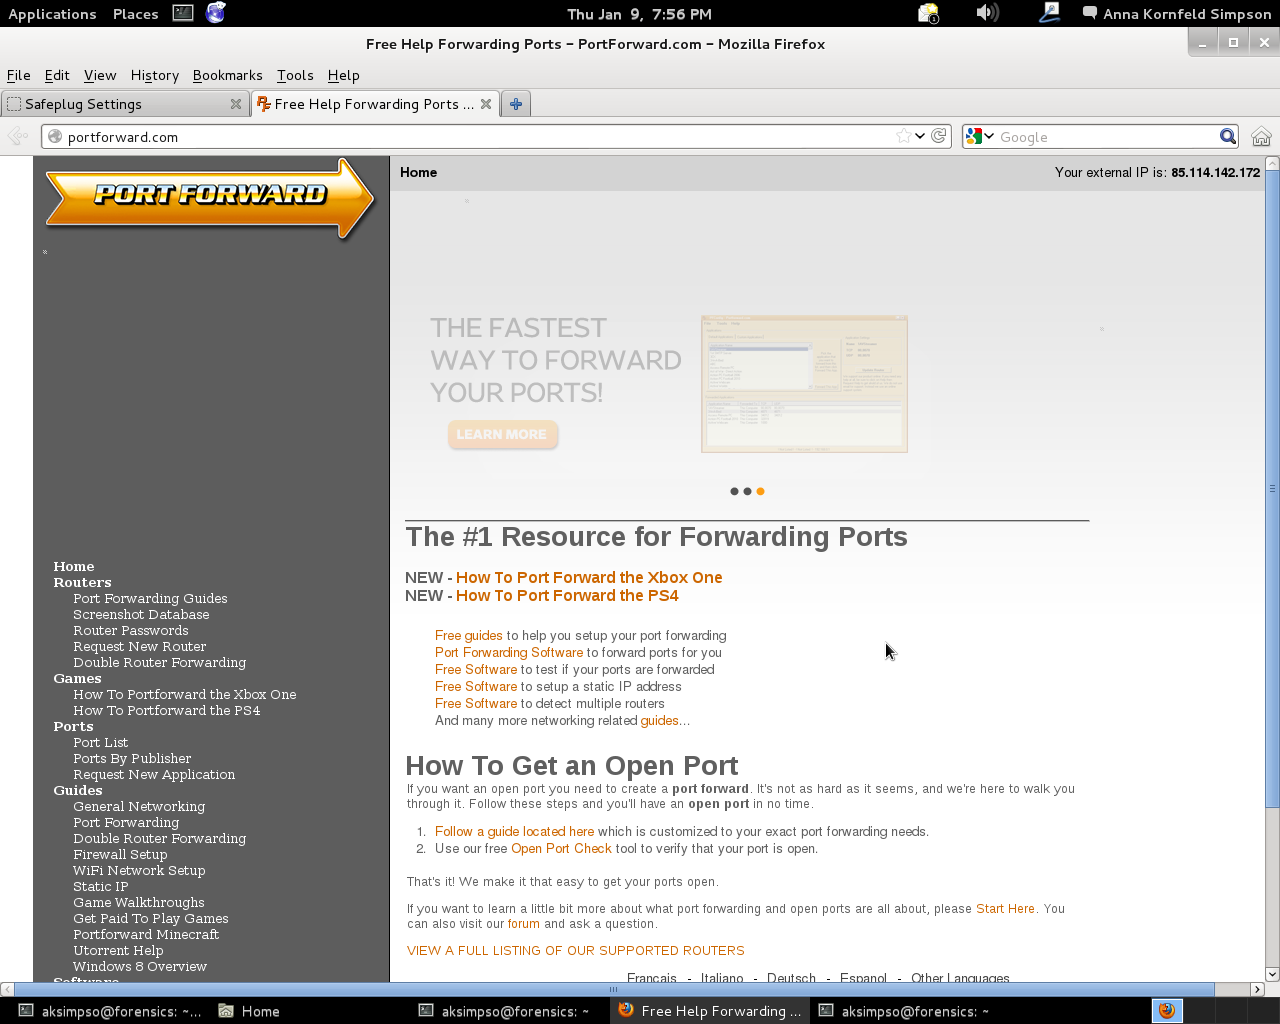
\includegraphics[width=.3\textwidth]{after}
  \label{fig:after}
}
\caption{Application of Safeplug proxy settings.}
\end{figure*}

Figure~\ref{fig:before} shows what a web page looks like before turning Tor and ad-blocking on, while Figure~\ref{fig:after} shows the same website after turning Tor and ad-blocking on.  Both of these figures show our IP address in the top right corner; due to the change in IP address we can see that our traffic is being routed through Tor.  

Next, we wanted to see how usable this would be to a normal Internet user.  A user would probably decide not to use Safeplug if they could not read their web pages (if they were not in their native language), or if they could not log into their accounts (some web sites will lock a user out if they try to log in from multiple countries in a short time period).  While browsing the Internet, we experienced some pages in German and Swedish, which is expected with Tor; if a user is not familiar with Tor, they may get frustrated and stop using Safeplug altogether.  We were also prompted with a request to ``Enter the name of the city where you usually sign in'' when we tried to log into our Google account, indicating that Google noticed we were trying to login from significantly ``unusual'' location.

\subsection{Cookies}  
While browsing the Internet, we logged into a Google Account in a tab, and then subsequently went to a website that had the Google+ widget in a different tab.  When we clicked on the Google+ widget, it remember who we are; so we can confirm that a cookie associated with the login was sent to the second Google+ page.  We experienced the same situation with Facebook and its corresponding ``like'' button.  This was confirmed by using FourthParty, a plugin developed by Jonathan Mayer at Stanford to collect information about cookies and other browsing data.

This is clearly not the perfect ``anonymity'' that Safeplug promised in their publicity.  Although normal use does follow this model of persisting logged in status across browser tabs and sessions, a user concerned about anonymity and seeing each session coming up differently (German vs Swedish) might mistakenly believe that they do not have to log out of their social media accounts to preserve their anonymity when accessing other websites.

More interesting and damaging to the user's control over their anonymity would be third-party cookies because the user cannot remove those just by logging out.  It requires a trip to the browser settings to clear cookies (or not have them set in the first place).  We used FourthParty to analyze the client's use of the Safeplug \cite{fourthparty}.  When collecting data on the existence of third-party cookies, we analyzed two separate browsing sessions; they were both new sessions with no cookies.  One of the sessions used the ad-block feature of the Safeplug and the other did not.  After analyzing data from Fourthparty, we found many third-party cookies in both sessions.  These included cookies from: abmr.net, bizographics.com, krxd.net, and bluekai.com among many others.  The ad-block functionality on the Safeplug reduced, but did not eliminate these third-party cookies.

Although Safeplug has a warning about clearing cookies on their FAQ page, it only mentions clearing cookies after a browser session.  Of greater concern would be tracking a user during their browser session from website to website; preventing this requires knowledge and constant vigilance from the user, or a browser that does not accept third-party cookies, such as the one provided in the Tor Browser Bundle.

\subsection{Browser Fingerprinting}
We used Panopticlick to examine the fingerprint of a freshly installed Firefox browser running through the Safeplug proxy~\cite{panopticlick}.  Panopticlick found the browser to be unique.  Fingerprinting is another way in which websites could correlate and de-anonymize user traffic without knowing the IP address.

\subsection{Latency}
If the latency of web requests using the Safeplug is noticeably longer than that of normal Internet use, users may be deterred from using the device.  Similarly, if turning Tor on, but not ad-blocking, adds a significant time delay, the user may only turn on the ad-blocking feature (without Tor).  We recorded the time for a web request on the following settings:

\begin{itemize}
\item Plain Firefox (traffic not running through the Safeplug device)
\item Firefox, no Tor, no ad-blocking (traffic running through the Safeplug device)
\item Firefox, Tor, no ad-blocking
\item Firefox, Tor, ad-blocking
\item Firefox, no Tor, ad-blocking
\item Tor Browser Bundle with Safeplug (all settings turned off)
\item Tor Browser Bundle
\end{itemize}

For each of the settings, we took 20 measurements; Figure~\ref{fig:latency2} shows the average time of a web request on each of the specified settings for three different web pages.  When taking these measurements, we loaded the page, but did not scroll; in many cases more objects are loaded when scrolling down a page.  The differences between web pages can most likely be attributed to the amount of advertisements and content running in plugins (such as video) on the web page.  

\begin{figure*}
  \centering
  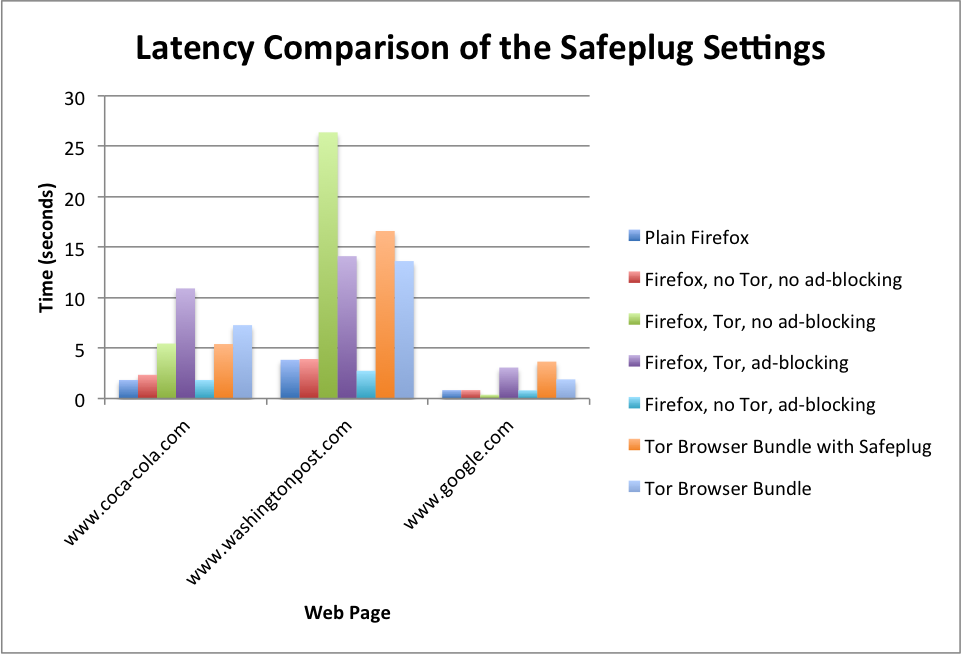
\includegraphics[width=0.7\textwidth]{graph2}
  \caption{Latency of web requests.}
  \label{fig:latency2}
\end{figure*}

It is interesting to note that the average web request time for accessing \url{www.washingtonpost.com} is greatest on the same settings that the average web request time for \url{www.google.com} is the least. This setting did not include ad-blocking, and therefore \url{www.washingtonpost.com} had to render each ad; \url{www.google.com} does not have any ads.  This also explains why the average latency was greater than the other settings for \url{www.washingtonpost.com}: each ad was requested through Tor.   

The latency of using the Safeplug with Firefox, Tor, and ad-blocking is comparable to that of using the Tor Browser Bundle.  For all three web pages, the Tor Browser Bundle had slightly lower latency; the Tor Browser Bundle blocks scripts, and for web pages such as \url{www.coca-cola.com}, this provides a significant latency decrease.  This, in conjunction with the fact that the Tor Browser Bundle is free and is issued directly from The Tor Project, shows a convincing argument to use the Tor Browser Bundle in place of the Safeplug.  

\section{Implementing Attacks}
As we discovered during the software analysis, the Safeplug has a remote procedure call (RPC) capability.  This is a script called \verb!xspctrl! found in \verb!/opt/xce/html/svc! and it contains various options.  Particularly, functional calls to this script include the ability to enable and disable for all of the Safeplug settings, including Tor, ad block, and Tor relay.  None of them require any arguments in the POST string.

\begin{figure*}
  \centering
  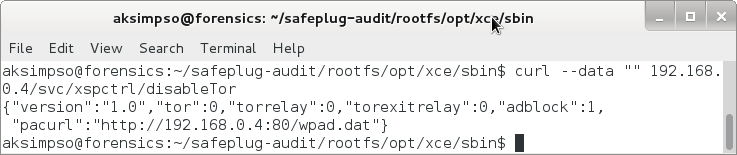
\includegraphics[width=.75\textwidth]{disabletor}
  \caption{Disabling Tor as an insider attack.}
  \label{disable}
\end{figure*}

\subsection{Insider Attack}
Since the Safeplug has no validation or authentication on the settings page or these RPC calls, any malicious party inside the network could easily modify the settings.  Such an adversary with a computer could load the Safeplug's settings page and adjust options such as disabling Tor or adding a site to the whitelist; since this page is meant to be accessible to normal Internet users, anyone can perform this attack.  Unlike many home routers, there is no username/password combination necessary to access this page.  

A more technically advanced user could send the call directly to the RPC server.  All the attacker would need to know is the IP address of the device.  It does not require SSH or discovering the (publically available) root password, or the user's new root password if they have been well-informed and adept enough to change it.  Figure \ref{disable} shows an example of the RPC version of this attack.

Since the RPC version of the attack just involves basic Internet tools (the ability to send a POST request), the attacker could also be any kind of device on the local network, or the local gateway if it is compromised.  The NSA ``Spymall'' catalog leaked in December shows tools for compromising a number of different devices and home routers are traditionally insecure \cite{spymall}.  It is easy to imagine any malicious party, not just one with the resources of a government (although governments might be some of the most interested parties in attacking a Tor proxy), compromising the gateway and using that access to make a disabling RPC call into the Safeplug.  This would occur silently from the perspective of a client unless they happen to check the settings page for the Safeplug.  Instead, the client would continue browsing with a belief that they are protected by their use of the Tor network, while in fact any external adversary can track their traffic.

This seems like a fairly important vulnerability and requires action from Pogoplug to fix.  Since the purpose of these RPC operations is unclear without access to more of the source code, it is possible that they could be disabled entirely.  If not, perhaps there is some authentication protocol that could be implemented.  The challenge of such a protocol from a user's point of view is that valid access would be infrequent so giving a user a password to remember would be a poor experience.

\subsection{CSRF Attack}
An external website can also perform this attack by returning a correctly formatted POST string via an internal user's browser.  This executes the same functionality as the Insider Attack, but the attacker does not need to be on the local network or know the IP address of the Safeplug.  The CSRF attack requires a nonmalicious insider user to visit a web page controlled by the attacker; additionally, the attacker must target the POST to the IP address of the Safeplug, but the attacker can get the right address by an exhaustive search.  We implemented this attack with less than 20 lines of Javascript code.  The following steps are necessary for the attack to be successful:

\begin{enumerate}
\item Set up a web page with the crafted Javascript code, which will send the POST request of the following format to all addresses in the common ranges: \url{http://<IP address>/svc/xspctrl/disableTor}.
\item Send the malicious link to a user in the targeted private network.
\item Once the user clicks the link and loads the malicious site, the correctly formatted POST request will be sent to every IP address in the ranges.  
\item Tor is disabled silently.  The user must check or refresh her settings page to learn that Tor is turned off.  
\end{enumerate}  

This exploits the RPC server in the same manner that the Insider Attack does.  While this attack requires a greater amount of time because the local IP address of the Safeplug must be guessed via search, the number of private address spaces is small, and the space likely to be occupied by a Safeplug on a home network is even smaller.  

The largest observed time to send requests to the 192.168.0.0/24 space was approximately 400 milliseconds; the entire attack costs approximately 800 milliseconds for sending requests to both 192.168.0.0/24 and 192.168.1.0/24 ranges - even when the website was being loaded over Tor.  In the case of a private network in the range of 172.16.0.0/16, the attack took less than 12 minutes (this generates script timeout warnings in most major browsers, which affects the timing of this attack).  This means that it would take a few hours to send requests to the full 172.16.0.0/12 range, which is commonly used in business networks.  The final private network space is 10.0.0.0/8 which is too large for an exhaustive search, but some simple optimization might make it feasible as well.  For example, using a GET request to get and parse the Safeplug settings page would allow the script to positively identify the Safeplug and stop the search.  However, the 192.168.0.0/24 and 192.168.1.0/24 ranges are much more common in home networks; because Safeplug is geared towards home network use, in most cases the script will take less than a second, a trivial amount of time for the attacker to spend.  

In addition to disabling Tor, the attacker can modify any other settings on the device.  This includes: enabling/disabling Tor, enabling/disabling ad-blocking, enabling/disabling the use of the device as a Tor relay node [note: this requires the user to do additional setup], enabling/disabling the use of the device as an exit node (if it is already a relay).  Lastly, the attacker can also modify the user's whitelist of sites that should not be routed through Tor.  This whitelist attack is particularly dangerous because the change is silent and much harder for the user to notice the addition of a single website to the whitelist than a global loss of Tor.  (Removal of a webpage from the whitelist is likely to cause usability problems and be more evident.)

\subsection{Gaining Access through SSH}
\label{sec:SSH}
    Another command available to the RPC server is enabling SSH to the device.  SSH instructions for Cloud Engine's other device (Pogoplug) are widely available online and an email in the Tor-talk mailing list confirms that the instructions are the same \cite{ceadmin}:
\begin{lstlisting}
curl --data ``'' http://<IP>/svc/xspctrl/enableSSHD
ssh root@<IP-of-Safeplug>
password: ceadmin
\end{lstlisting}

Having a publically available root password means that SSH can be done effectively without authentication.  We tried the SSH procedure twice, once before the Internet connection and activation, and once afterwards.  Before the activation and update procedure, SSH was not available.  The simple \verb!Hbplug! software on the box could not accept this RPC call.  However, once the box was updated and had Lighttpd installed, the SSH procedure was available and we could download the contents of the root filesystem for analysis.

\subsection{Spoofing the Update Server}
\label{dnsspoof}
A more dangerous class of vulnerabilities comes from the fact that the update process happens over insecure TCP rather than any kind of encrypted process.  During our network analysis of the activation process, we discovered that the update script is downloaded via TCP from an IP address provided by the Pogoplug servers.  This update script (run as root) then downloads the Safeplug's software (Tor, Privoxy, Lighttpd, and wget) and checks it against MD5 hashes, but it is not clear whether there is suitable verification of the update script itself.  An adversary could use DNS spoofing or compromise the Pogoplug server in order to force users to download a malicious update script - for example, something that turns the Safeplug into a surveillance box while appearing to provide the correct functionality.  Since the most efficient way to check this would be to verify the contents of the Safeplug box itself by SSHing in, it is clear that any kind of mitigation to this attack would be beyond an average user.  Because the activation occurs over TCP rather than anything more secure, an adversary who can spoof DNS replies to the user has a paved gateway into the Safeplug box.  This turns a device that does not live up to expectations, but is otherwise harmless, into something that actively harms security on the network.

\section{Related Work}
To our knowledge, there has been no other study analyzing the security of Pogoplug's Safeplug device.  However there has been much prior research on the primary technology that the device uses: Tor.  Additionally, the security vulnerabilities that Safeplug attempts to secure users against have been previously studied in great detail; these include fingerprinting and cookies.  

{\bf Tor.} Prior security evaluations of the Tor network reveal a myriad of potential vulnerabilities.  A significant area of research on Tor relates to diversity of autonomous systems (ASes).  Feamster and Dingledine argue that a user's anonymity may be compromised by using geographically diverse ASes; when analyzing both sides of an anonymous path, it is more likely the same AS will appear in both sides of a long path than in a short path~\cite{feamster}.  Murdoch and Zielinski also argue against AS diversity.  They state that AS diversity does not improve security because traffic is routed through ASes at Internet exchange points (IXPs); therefore, an IXP can observe traffic that passes through multiple ASes~\cite{murdoch2}.  There has also been proven traffic correlation attacks that are efficient on the Tor network~\cite{murdoch, overlier}.  Johnson, Wacek, Jansen, Sherr, and Syverson evaluated Tor's security against reasonably realistic adversaries and contribute metrics that model security over time.  They found that in a period of six months, 80\% of all users may be deanonymized by a reasonably realistic Tor-relay adversary.  Johnson et al. take into account how the Tor network evolves over time when evaluating Tor's security~\cite{tor2}.  While Safeplug does not introduce or modify how Tor is used, it routes all traffic through the Tor network; Safeplug is also vulnerable to the attacks found in prior research on Tor.  

{\bf Fingerprinting.}  Website fingerprinting attacks as well as remote physical device fingerprinting attacks have shown they can identify users, even when specific defenses have been used in order to prevent them. Previous research has shown that web page fingerprinting attacks are possible~\cite{dyer, herrmann, panchenko}.  Cai, Zhang, Joshi, and Johnson introduced both a web page and website fingerprinting attack that defeats many recently proposed defenses, including cover traffic and randomized pipeling.  They find that their attack is successful 83.7\% of the time when the defense is the use of Tor; the success rate decreases to 52.2\% when the defense is the use of Tor, randomized pipelining, padding packets to 1500 bytes, and adding cover traffic at a 1:1 ratio~\cite{fingerprint1}.  These results can be extended to the security of Safeplug.  Because Safeplug uses only Tor to anonymize users, it may be susceptible to this type of fingerprinting attack.

{\bf Cookies} There has been much policy and technology debate around the topic of third-party web tracking.  Mayer and Mitchell survey recent policy and technology stances on web tracking; while tracking allows for free web content and innovation, it compromises a user's privacy~\cite{commercial2}.  They discuss the existence and use of stateful tracking by using ``supercookies.''  While many companies use cookies, there has also been work in developing privacy-preserving third-party services, such as Privad, Adnostic, and RePriv~\cite{guha, toubiana, fredrikson}.

\section{Discussion}
\subsection{Engineering Fixes}
The most critical engineering fix is authentication in the POST calls to prevent the CSRF attack.  A typical approach to preventing CSRF attacks is using a cookie and a hidden form field set in the settings page of the Safeplug hosts; the cookie must be returned by the browser when making the POST request to the RPC server \cite{csrfdef}.  Although someone doing a CSRF attack such as the one described above could get the cookie sent, because of the same-origin policy, the adversary would not be able to examine the contents of the cookie to determine what to put in the form field.

\subsection{Structural Problems}
However, there are much more significant structural problems with implementing a Tor connection via an HTTP proxy.  Several of the usability problems involve user awareness and vigilance.  For example, cookies and fingerprinting problems mean that users could still be tracked across websites, regardless of whether the ad-block functionality on the Safeplug is enabled.  This poses an unreasonable stress on users who must be aware of their browsing practices and does not bode well for the advertised security and anonymity.

One type of client that deserves special attention is a non-Android mobile phone user.  Although the Tor Project publishes an Android app called Orbot on the Android Market, which is supported for Android versions 2.3 and later, there are no official Tor apps for iPhones or other non-Android devices~\cite{orbot,amorbot}.  Safeplug provides proxy functionality and instructions for Safari on the iPhone; however, this would only work while the user is on that wifi network that the Safeplug routes through.  If any data is sent over the cellular network or another wifi network, then the security of Tor is lost.  Additionally, the user may have to disable the proxy whenever they move to a different network, and remember to re-enable it when they want to use Tor.  This is certainly not transparent usability.  Users who are truly concerned about anonymity online should eschew the Safeplug and purchase a device that supports the Tor Browser Bundle or other Tor Project software.

\subsection{Opportunities}
Despite all the structural problems, is there a market for a Torifying piece of hardware?  Given the security pitfalls in comparison to a piece of software such as the Tor Browser Bundle, there seems to be no reason for a user that can run the Tor Browser Bundle to purchase the Safeplug or any other device.  For mobile phones, the proxy problems with mobility contribute to an already high usability cost.  However, there are an emerging class of ``smart home'' devices which may connect to the Internet.  It is possible that some of these devices can be configured to use an HTTP proxy or some other middle box to Torify their traffic to an external service provider.  For them, is the benefit of some anonymity via a Safeplug-like device worthwhile?  Since the data sent by these devices to the service provider likely contains identifying information, the use of Tor probably only protects the user's location at the expense of connection time and load on the Tor network.  Since proxy configuration on such devices is likely to be difficult and the amount of information hidden is unlikely to be worth the effort, a Torifying box that functions as a proxy has questionable use in this space as well.

\section{Conclusion}
Ultimately, the structural concerns of the Safeplug ``Torifying proxy-in-a-box'' strategy indicate that this is problematic as a method for security and anonymity online.  It is critical for Safeplug to correct their engineering errors, particularly the vulnerability to silently disable Tor, in order to protect customers who have already made use of the device, but users who are truly concerned about safety and anonymity online should make use of technologies directly from the Tor Project.


% Note that IEEE does not put floats in the very first column - or typically
% anywhere on the first page for that matter. Also, in-text middle ("here")
% positioning is not used. Most IEEE journals/conferences use top floats
% exclusively. Note that, LaTeX2e, unlike IEEE journals/conferences, places
% footnotes above bottom floats. This can be corrected via the \fnbelowfloat
% command of the stfloats package.

% conference papers do not normally have an appendix


% trigger a \newpage just before the given reference
% number - used to balance the columns on the last page
% adjust value as needed - may need to be readjusted if
% the document is modified later
%\IEEEtriggeratref{8}
% The "triggered" command can be changed if desired:
%\IEEEtriggercmd{\enlargethispage{-5in}}

% references section

% can use a bibliography generated by BibTeX as a .bbl file
% BibTeX documentation can be easily obtained at:
% http://www.ctan.org/tex-archive/biblio/bibtex/contrib/doc/
% The IEEEtran BibTeX style support page is at:
% http://www.michaelshell.org/tex/ieeetran/bibtex/
%\bibliographystyle{IEEEtran}
% argument is your BibTeX string definitions and bibliography database(s)
%\bibliography{IEEEabrv,../bib/paper}
%
% <OR> manually copy in the resultant .bbl file
% set second argument of \begin to the number of references
% (used to reserve space for the reference number labels box)
\begin{thebibliography}{1}

\bibitem{spymall} Appelbaum et. al. ``Shopping for Spy Gear: Catalog Advertises 
NSA Toolbox'' \emph{Der Spiegel} 29 December 2013 \url{www.spiegel.de/internatio
nal/world/catalog-reveals-nsa-has-back-doors-for-numerous-devices-a-940994.html}

\bibitem{archforum} Arch Linux ARM Forums. ``Installation on the Pogoplug Series 4.'' \url{http://archlinuxarm.org/forum/viewtopic.php?f=3&t=2284&start=14&sid=11c74c51b7bab241186a8341ba953095}

\bibitem{nsa} Arther, Charles.  ``NSA scandal: what data is being monitored and how does it work?'' \url{http://www.theguardian.com/world/2013/jun/07/nsa-prism-records-surveillance-questions}.

\bibitem{fingerprint1} Cai, Xiang, et al. ``Touching from a distance: Website fingerprinting attacks and defenses.'' \emph{Proceedings of the 2012 ACM conference on Computer and Communications Security (CCS)}, 2012.

\bibitem{ceadmin} Colleton, Lee. ``Fwd: SSH on Safeplug'' \emph{Tor-talk mailing list} 2 January 2014. \url{http://archives.seul.org/or/talk/Jan-2014/msg00003.html}

\bibitem{tor} Dingledine, Roger, et. al. ``Tor: The second-generation onion router.'' \emph{USENIX Security Symposium}, 2004.

\bibitem{dyer} Dyer, Kevin P., Coull, Scott E., Ristenpart, Thomas, and Shrimpton, Thomas.  ``Peek-a-boo, i still see you: Why efficient traffic analysis countermeasures fail.'' \emph{In Proceedings of the 33rd Annual IEEE Symposium on Security and Privacy}, 2012.

\bibitem{panopticlick} Electronic Fronteir Foundation. ``Panopticlick.'' \url{https://panoptlick.eff.org}

\bibitem{feamster} Feamster, Nick, and Dingledine, Roger.  ``Location Diversity in Anonymity Networks.''  \emph{In ACM Workshop on Privacy in the Electronic Society (WPES)}, 2004.

\bibitem{fredrikson} Fredrikson, M., and Livshits, B. ``Repriv: Re-envisioning in-browser privacy.'' \emph{In Proceedings of the 2011 IEEE Symposium on Security and Privacy}, May 2011.

\bibitem{guha} Guha, S., Cheng, B., and Francis, P. ``Privad: Practical privacy in online advertising.'' \emph{In Proceedings of the 2011 USENIX Symposium on Networked Systems Design and Implementation}, April 2011.

\bibitem{bittech} Halfacree, Gareth. ``Pogoplug launches Tor-powered Safeplug'' \emph{bit-tech.net} 25 November 2013, \url{http://www.bit-tech.net/news/hardware/2013/11/25/pogoplug-safeplug/1}.

\bibitem{herrmann} Herrmann, Dominik, Wendolsky, Rolf, and Federrath, Hannes.  ``Website fingerprinting: attacking popular privacy enhancing technologies with the multinomial naive-bayes classifier.'' \emph{In Proceedings of the 2009 ACM workshop on Cloud computing security}.

\bibitem{tor2} Johnson, Aaron, et al. ``Users get routed: Traffic correlation on Tor by realistic adversaries.'' \emph{Proceedings of the 2013 ACM SIGSAC conference on Computer \& Communications Security (CCS)}, 2013.

\bibitem{dropbear} Johnston, Matt. ``Dropbear SSH.'' \url{https://matt.ucc.asn.au/dropbear/dropbear.html}

\bibitem{fingerprint2} Kohno, Tadayoshi et. al. "Remote physical device fingerprinting." Dependable and Secure Computing, IEEE Transactions on 2.2 (2005): 93-108.

\bibitem{law} The Legal FAQ for Tor Relay Operators. \url{https://www.torproject.org/eff/tor-legal-faq}.

\bibitem{lighttpd} Lighttpd. \url{http://www.lighttpd.net}


\bibitem{marvellhw} Marvell, ``88F6190 and 88F6192 Integrated Controller Hardware Specifications'' 2 December 2008. \url{http://www.marvell.com//embedded-processors/kirkwood/assets/HW_88F619x_OpenSource.pdf}

\bibitem{marvell} Marvell, ``Marvell 88F6192 SoC with Sheeva Technology'' 2009. \url{http://www.marvell.com//embedded-processors/kirkwood/assets/88F6192-003_ver1.pdf}

\bibitem{marvell2} Marvell, ``Marvell Alaska 88E1116R'' 2007. \url{http://www.marvell.com/transceivers/assets/Marvell-Alaska-88E1116R-Single-Port-GbE.pdf}

\bibitem{fourthparty} Mayer, Jonathan. ``FourthParty'' \url{http://fourthparty.info}

\bibitem{commercial2} Mayer, Jonathan R., and John C. Mitchell. "Third-party web tracking: Policy and technology." \emph{IEEE Symposium on Security and Privacy (SP)}, 2012.

\bibitem{gigaom} Meyer, David. ``Say hello to Safeplug, Pogoplug’s \$49 Tor-in-a-box for anonymous surfing'', \emph{GigaOm}, 21 November 2013. \url{http://gigaom.com/2013/11/21/say-hello-to-safeplug-pogoplugs-49-tor-in-a-box-for-anonymous-surfing/}.

\bibitem{murdoch} Murdoch, S.J., Danezis, G.  ``Low-Cost Traffic Analysis of Tor.'' \emph{In IEEE Symposium on Security and Privacy (Oakland)}, 2005.

\bibitem{murdoch2} Murdoch, S.J. and Zielinski, P.  ``Sampled Traffic Analysis by Internet-Exchange-Level Adversaries.'' \emph{In Privacy Enhancing Technologies (PET)}, 2007.

\bibitem{overlier} Overlier, L. and Syverson, P.  ``Locating Hidden Servers.'' \emph{In IEEE Symposium on Security and Privacy (Oakland)}, 2006.

\bibitem{panchenko} Panchenko, Andriy, Niessen, Lukas, Zinnen, Andreas, and Engel, Thomas.  ``Website fingerprinting in onion routing based anonymization networks.'' \emph{In Proceedings of the 10th Workshop on Privacy in the Electronic Society}, 2011.

\bibitem{pano} Panopticlick. \url{https://panopticlick.eff.org/}.

\bibitem{pew} Pew Research Center.  ``Anonymity, Privacy, and Security Online.'', \url{http://www.pewinternet.org/files/old-media//Files/Reports/2013/PIP_AnonymityOnline_090513.pdf}.

\bibitem{pogo} Pogoplug. ``Pogoplug'', \url{https://pogoplug.com}.

\bibitem{safeplug} Pogoplug. ``Safeplug'', \url{https://pogoplug.com/safeplug}.

\bibitem{privoxy} Privoxy. \url{https://www.privoxy.org}

\bibitem{schneier} Schneier, Bruce. ``Tor Appliance.'' \emph{Schneier on Security}, 27 November 2013. \url{https://www.schneier.com/blog/archives/2013/11/tor_appliance.html}.

\bibitem{kernelcve} Security Database. ``Linux Linux Kernel 2.6.13.8 CVE'' \url{http://www.security-database.com/cpe.php?detail=cpe:/o:linux:linux_kernel:2.6.31.8}

\bibitem{techreview} Simonite, Tom. ``Online Anonymity in a Box, for \$49'', \emph{MIT Technology Review}, 21 November 2013. \url{http://www.technologyreview.com/news/521676/online-anonymity-in-a-box-for-49/}.

\bibitem{pogo4} SmallNetBuilder. ``Pogoplug Series 4 Reviewed.'' \url{http://www.smallnetbuilder.com/cloud/cloud-storage/486-pogoplug-series-4-reviewed}

\bibitem{wired} Solon, Olivia. ``Safeplug makes it super-easy to harness Tor\'s anonymity at home,'' \emph{Wired UK}, 22 November 2013. \url{http://www.wired.co.uk/news/archive/2013-11/22/safeplug-tor}.

\bibitem{tormailinglist} Tor Mailing List.  \url{https://lists.torproject.org/pipermail/tor-talk/2013-November/031199.html}.

\bibitem{orbot} ``Tor on Android.'' \emph{Tor Project.} Accessed February 2014. \url{https://torproject.org/docs/android.html.en}

\bibitem{torproject} The Tor Project.  \url{https://www.torproject.org/}.

\bibitem{amorbot} The Tor Project. ``Orbot: Proxy with Tor.'' \emph{Google Android Market}. Accessed 7 February 2014, \url{https://play.google.com/store/apps/details?id=org.torproject.android}

\bibitem{toubiana} Toubiana, V., Narayanan, A., Boneh, D., Nissenbaum, H., and Barocas, S. ``Adnostic: Privacy preserving targeted advertising.'' \emph{In Proceedings of the 2010 Network and Distributed System Security Symposium}, March 2010.

\bibitem{wireshark} Wireshark, \url{http://www.wireshark.org/}. 

\bibitem{csrfdef} Zeller and Felten. ``Cross-Site Request Forgeries: Exploitation and Prevention.'' \emph{Princeton Technical Report}. 2008.


\end{thebibliography}




% that's all folks
\end{document}


